\documentclass[acmlarge]{acmart}

% --- Course-report front matter: no ACM rights block / reference-format box ---
\setcopyright{none}
\settopmatter{printacmref=false}
\renewcommand\footnotetextcopyrightpermission[1]{}
\pagestyle{plain}
\AtBeginDocument{\fancyfoot[RO,LE]{}\fancypagestyle{firstpagestyle}{\fancyhf{}\renewcommand{\headrulewidth}{0pt}}}

\usepackage{booktabs}
\usepackage{array}
\usepackage{enumitem}
\setlist{nosep,leftmargin=1.4em}

\newcommand{\evs}[1]{\textsc{#1}}
\newcommand{\runin}[1]{\par\addvspace{4pt}\noindent\hspace{\parindent}\textit{#1}\hspace{0.45em}\ignorespaces}

% All numbers below are macros generated from results/ by src/make_report_tables.py
% Generated by src/make_report_tables.py from results/. Do not edit by hand.
\newcommand{\nTune}{400}
\newcommand{\nDev}{350}
\newcommand{\nTrain}{399}
\newcommand{\nTrainSampled}{400}
\newcommand{\nPool}{749}
\newcommand{\nDecFailed}{1}
\newcommand{\nParseFailed}{0}
\newcommand{\nPoolS}{201}
\newcommand{\nPoolR}{441}
\newcommand{\nPoolC}{50}
\newcommand{\nPoolN}{57}
\newcommand{\majorityAcc}{0.589}
\newcommand{\exclTotalDev}{500}
\newcommand{\exclKeptDev}{363}
\newcommand{\exclTotalTrain}{1000}
\newcommand{\exclKeptTrain}{800}
\newcommand{\unvPool}{73}
\newcommand{\unvTuneK}{73}
\newcommand{\yesPool}{13}
\newcommand{\noPool}{13}
\newcommand{\chosenK}{3}
\newcommand{\chosenM}{2}
\newcommand{\chosenTau}{0.25}
\newcommand{\chosenClf}{gradient boosting}
\newcommand{\chosenCal}{isotonic}
\newcommand{\tuneCVsplits}{5}
\newcommand{\tuneFoneLRthree}{0.2438}
\newcommand{\tuneFoneLRfive}{0.2437}
\newcommand{\tuneFoneGBthree}{0.270}
\newcommand{\tuneAccGBthree}{0.328}
\newcommand{\tuneECEiso}{0.054}
\newcommand{\tuneECEtemp}{0.105}
\newcommand{\tuneECEnone}{0.246}
\newcommand{\tuneStateAccTwo}{0.240}
\newcommand{\tuneTauCov}{59.5}
\newcommand{\aurocMarginThree}{0.652}
\newcommand{\aurocMarginFive}{0.645}
\newcommand{\aurocMarginEight}{0.651}
\newcommand{\goldRefF}{0.377}
\newcommand{\vThreeDF}{$-$0.011}
\newcommand{\vThreeDAUROC}{$-$0.021}
\newcommand{\vThreeUnvBase}{73}
\newcommand{\vThreeUnvVar}{60}
\newcommand{\accPool}{0.287}
\newcommand{\accPoolLo}{0.255}
\newcommand{\accPoolHi}{0.319}
\newcommand{\accDev}{0.329}
\newcommand{\accTrain}{0.251}
\newcommand{\mfPool}{0.225}
\newcommand{\mfPoolLo}{0.196}
\newcommand{\mfPoolHi}{0.256}
\newcommand{\mfDev}{0.260}
\newcommand{\mfTrain}{0.194}
\newcommand{\eceRawPool}{0.261}
\newcommand{\eceRawPoolLo}{0.232}
\newcommand{\eceRawPoolHi}{0.293}
\newcommand{\eceRawDev}{0.237}
\newcommand{\eceRawTrain}{0.285}
\newcommand{\eceCalPool}{0.038}
\newcommand{\eceCalPoolLo}{0.030}
\newcommand{\eceCalPoolHi}{0.072}
\newcommand{\eceCalDev}{0.078}
\newcommand{\eceCalTrain}{0.057}
\newcommand{\brierRawPool}{0.790}
\newcommand{\brierRawPoolLo}{0.757}
\newcommand{\brierRawPoolHi}{0.823}
\newcommand{\brierRawDev}{0.777}
\newcommand{\brierRawTrain}{0.800}
\newcommand{\brierCalPool}{0.701}
\newcommand{\brierCalPoolLo}{0.678}
\newcommand{\brierCalPoolHi}{0.724}
\newcommand{\brierCalDev}{0.716}
\newcommand{\brierCalTrain}{0.687}
\newcommand{\stateAccPool}{0.236}
\newcommand{\stateAccPoolLo}{0.207}
\newcommand{\stateAccPoolHi}{0.266}
\newcommand{\stateAccDev}{0.269}
\newcommand{\stateAccTrain}{0.208}
\newcommand{\covPZero}{100.0}
\newcommand{\riskPZero}{71.3}
\newcommand{\unsafePZero}{24.8}
\newcommand{\unsafePZeroLo}{21.8}
\newcommand{\unsafePZeroHi}{27.8}
\newcommand{\covPOne}{53.8}
\newcommand{\riskPOne}{59.1}
\newcommand{\unsafePOne}{19.5}
\newcommand{\unsafePOneLo}{16.6}
\newcommand{\unsafePOneHi}{22.3}
\newcommand{\covPTwo}{35.1}
\newcommand{\riskPTwo}{63.5}
\newcommand{\unsafePTwo}{13.5}
\newcommand{\unsafePTwoLo}{11.1}
\newcommand{\unsafePTwoHi}{15.9}
\newcommand{\covPThree}{24.8}
\newcommand{\riskPThree}{54.8}
\newcommand{\unsafePThree}{11.1}
\newcommand{\unsafePThreeLo}{8.9}
\newcommand{\unsafePThreeHi}{13.4}
\newcommand{\covPFourA}{35.1}
\newcommand{\riskPFourA}{53.6}
\newcommand{\unsafePFourA}{12.0}
\newcommand{\unsafePFourALo}{10.0}
\newcommand{\unsafePFourAHi}{15.1}
\newcommand{\covPFourB}{24.8}
\newcommand{\riskPFourB}{47.3}
\newcommand{\unsafePFourB}{9.7}
\newcommand{\unsafePFourBLo}{7.7}
\newcommand{\unsafePFourBHi}{11.7}
\newcommand{\dRiskThreeZero}{$-$16.5}
\newcommand{\dRiskThreeZeroLo}{$-$22.5}
\newcommand{\dRiskThreeZeroHi}{$-$10.5}
\newcommand{\dUnsafeThreeZero}{$-$13.8}
\newcommand{\dUnsafeThreeZeroLo}{$-$16.3}
\newcommand{\dUnsafeThreeZeroHi}{$-$11.5}
\newcommand{\dRiskTwoFourA}{+9.9}
\newcommand{\dRiskTwoFourALo}{+4.2}
\newcommand{\dRiskTwoFourAHi}{+16.3}
\newcommand{\dUnsafeTwoFourA}{+1.5}
\newcommand{\dUnsafeTwoFourALo}{$-$1.2}
\newcommand{\dUnsafeTwoFourAHi}{+3.3}
\newcommand{\dRiskThreeFourB}{+7.5}
\newcommand{\dRiskThreeFourBLo}{0.0}
\newcommand{\dRiskThreeFourBHi}{+15.1}
\newcommand{\dUnsafeThreeFourB}{+1.3}
\newcommand{\dUnsafeThreeFourBLo}{$-$0.4}
\newcommand{\dUnsafeThreeFourBHi}{+3.3}
\newcommand{\dRiskTwoFourADev}{+8.7}
\newcommand{\dUnsafeThreeZeroDev}{$-$13.1}
\newcommand{\covPThreeDev}{28.6}
\newcommand{\dRiskTwoFourATrain}{+12.8}
\newcommand{\dUnsafeThreeZeroTrain}{$-$14.3}
\newcommand{\covPThreeTrain}{21.6}
\newcommand{\aurocConf}{0.708}
\newcommand{\aurocConfState}{0.707}
\newcommand{\dAuroc}{$-$0.001}
\newcommand{\dAurocLo}{$-$0.018}
\newcommand{\dAurocHi}{+0.016}
\newcommand{\brierConf}{0.180}
\newcommand{\brierConfState}{0.178}
\newcommand{\aurc}{0.562}
\newcommand{\stateShareSup}{25.1}
\newcommand{\stateAccSup}{31.4}
\newcommand{\stateNSup}{188}
\newcommand{\stateShareRef}{10.0}
\newcommand{\stateAccRef}{49.3}
\newcommand{\stateNRef}{75}
\newcommand{\stateShareMix}{16.2}
\newcommand{\stateAccMix}{51.2}
\newcommand{\stateNMix}{121}
\newcommand{\stateShareIns}{48.7}
\newcommand{\stateAccIns}{15.6}
\newcommand{\stateNIns}{365}
\newcommand{\refStateGoldR}{81}
\newcommand{\predC}{265}
\newcommand{\predN}{110}
\newcommand{\foneC}{0.114}
\newcommand{\foneN}{0.108}
\newcommand{\unsafeZeroS}{33}
\newcommand{\unsafeThreeS}{10}
\newcommand{\unsafeZeroR}{16}
\newcommand{\unsafeThreeR}{9}
\newcommand{\unsafeZeroC}{42}
\newcommand{\unsafeThreeC}{22}
\newcommand{\unsafeZeroN}{51}
\newcommand{\unsafeThreeN}{18}
\newcommand{\unsafeErrTotal}{186}
\newcommand{\postRuleAcc}{0.506}
\newcommand{\postClfAcc}{0.365}
\newcommand{\postAgree}{46.8}
\newcommand{\postN}{263}
\newcommand{\taxEv}{11}
\newcommand{\taxNua}{8}
\newcommand{\taxMis}{4}
\newcommand{\taxClf}{3}
\newcommand{\taxDec}{3}
\newcommand{\taxCons}{1}
\newcommand{\taxPol}{1}
\newcommand{\taxGold}{1}
\newcommand{\taxTotal}{32}
\newcommand{\bootN}{2000}
\newcommand{\modelDigest}{845dbda0ea48}


\begin{document}

\title{Beyond the Verdict: Evidence States and Calibrated Abstention in Evidence-First Fact-Checking (Short-Term Project 1, Model-Level Pilot)}

\author{Taha Mehdi}
\email{taha.mehdi@sabanciuniv.edu}
\authornote{Student ID: 33731.}
\affiliation{%
  \institution{Sabanc{\i} University, CS 48013 / CS 58013}
  \department{Human-Centered Artificial Intelligence, Fall 2026--27 (Project 5)}
  \city{Istanbul}
  \country{T{\"u}rkiye}}

\begin{abstract}
Fact-checking pipelines that always return a verdict hide missing or conflicting evidence. This pilot tests, at model level only, whether an explicit \emph{evidence state} (supports, refutes, mixed, insufficient) derived from an explainable pipeline's per-question answers, combined with calibrated abstention, lets a system withhold verdicts it should not give. On \nPool{} AVeriTeC claims, withholding cuts wrong decisive verdicts (``unsafe errors'') from \unsafePZero\% to \unsafePThree\% of claims, but only \covPThree\% of claims are answered. Much of this drop is mechanical: withholding a random \covPThree\% sample of the baseline's answers would give about \randRefPThree\%, and among the claims P3 answers, \ansUnsafePThree\% are unsafe errors (baseline \ansUnsafePZero\%). The mechanism check is negative: withholding by state is no better than withholding by calibrated confidence at the same rate, and the state adds no information about verdict correctness beyond confidence. The verdict classifier itself is weak (macro-F1 \mfPool), which coincides with \unvPool\% Unverified answers; no oracle-evidence run tests the cause. Nothing here measures a benefit for human users.
\end{abstract}

\ccsdesc[500]{Human-centered computing~Empirical studies in HCI}
\ccsdesc[300]{Computing methodologies~Natural language processing}
\keywords{fact-checking, uncertainty communication, abstention, appropriate reliance, human oversight}

\maketitle

%==========================================================================
\section{Project Topic and Task; Intended Users and Context}\label{sec:task}
%==========================================================================
\runin{Task.} The model-level task is four-way claim verification on AVeriTeC~\cite{schlichtkrull2023}: given a claim and a per-claim knowledge store of web documents, predict Supported (S), Refuted (R), Conflicting Evidence/Cherry-picking (C) or Not Enough Evidence (N). The pipeline follows the explainable, question-based design of Alto\`e et al.~\cite{altoe2025} (decompose the claim into yes/no questions, retrieve evidence, answer per question, map the answer counts to a verdict), implemented with an open-weight model. The reader sees the evidence state together with the verdict, or the state alone when the verdict is withheld.

\runin{Intended users and who is affected.} Intended users, as in the surveyed human-centered fact-checking work~\cite{nakov2021}, are people who must judge a model-produced verdict before relying on it: junior fact-checkers, journalists, media-literacy students and moderators. Affected people also include those whose claims are labelled, and readers downstream of any published check. The decision the output may inform is \emph{accept, check further, or escalate}. This pilot studies the model component only; no users took part.

\runin{Context and out-of-scope use.} English claims from a fixed public benchmark with a static evidence store. The system is decision support, not an authority; it should not be used for automated moderation or on the sensitive topics excluded here (Section~\ref{sec:data}).

%==========================================================================
\section{Human-Centered Objective and Design Rationale}\label{sec:objective}
%==========================================================================
\runin{Principle.} Uncertainty communication and human oversight, aimed at \emph{appropriate} reliance: a reader should be told when a verdict rests on missing or contradictory evidence instead of receiving a fluent forced label. Forced verdicts are least warranted exactly on claims whose evidence is missing or conflicting, which AVeriTeC labels N and C, and explanations can raise acceptance of wrong outputs~\cite{bansal2021,si2024}.

\runin{Mechanism.} Two additions to the same pipeline: (i) an \emph{evidence state} computed by transparent rules from the six answer counts, and (ii) an \emph{abstention policy} that withholds the headline verdict when calibrated confidence is low or the state is \evs{Mixed} or \evs{Insufficient}.

\runin{Observable (model-level) evidence, fixed before any result} (\texttt{docs/DESIGN\_LOCK.md}): (i) the state predicts verdict errors beyond calibrated confidence; (ii) withholding lowers the rate of wrong decisive verdicts at an acceptable coverage cost; (iii) withholding by state beats withholding by a confidence threshold at the \emph{same} withhold rate. A pre-set interpretation matrix says that if the state adds no information beyond confidence, it is reported as redundant. These are proxies: they cannot show that people decide better.

%==========================================================================
\section{Baseline and Proposed Pipeline Design}\label{sec:design}
%==========================================================================
\begin{figure}[t]
  \centering
  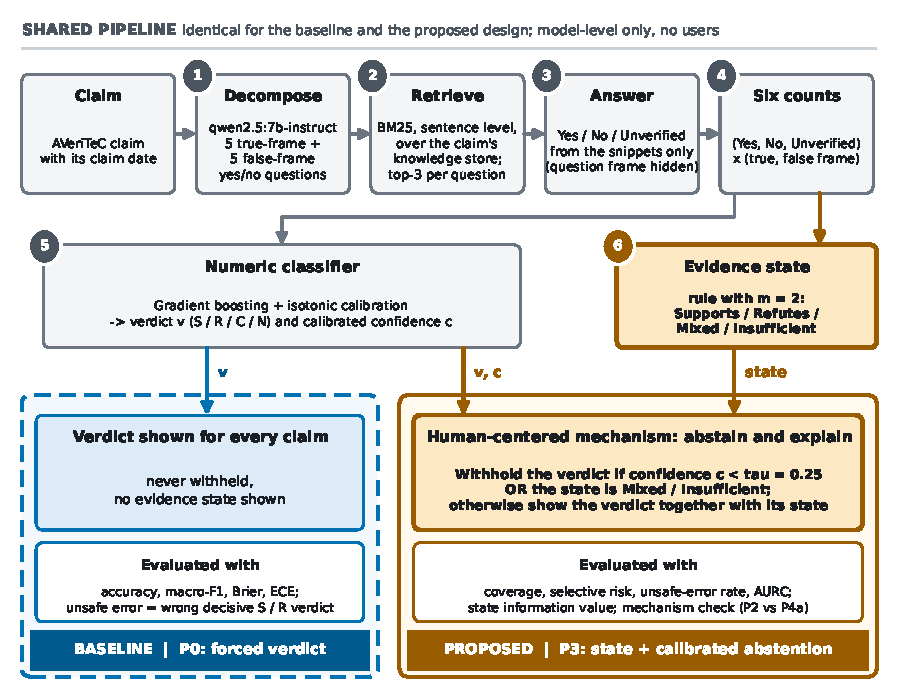
\includegraphics[width=0.88\linewidth]{figures/pipeline.pdf}
  \caption{Pipeline. Stages 1--5 are shared. The \textbf{baseline} (blue) always shows the verdict; the \textbf{proposed design} (orange) adds the evidence state (stage 6) and the abstention rule, which is the human-centered mechanism.}
  \label{fig:pipeline}
\end{figure}

\runin{Shared pipeline (Figure~\ref{fig:pipeline}).} (1) Qwen2.5-7B-Instruct writes 10 yes/no questions per claim: 5 \emph{true-frame} (``Yes'' is consistent with the claim) and 5 \emph{false-frame} (``Yes'' is consistent with it being false). (2) Sentence-level BM25~\cite{robertson2009} over the claim's store returns the top-\chosenK{} sentences per question; the store's gold-document flag is never used. (3) The same model answers each question Yes/No/Unverified from the snippets only; it never sees the claim or the frame. (4) Answers are summarised as six counts (Yes, No, Unverified) $\times$ (true, false frame). (5) A classifier (\chosenClf, class-balanced) maps the counts to a four-way verdict and a probability; the confidence $c$ is the calibrated probability of the predicted class (\chosenCal{} regression fitted on out-of-fold tuning predictions).

\runin{Evidence state (stage 6).} With $\textit{sup}=$ true-frame Yes $+$ false-frame No and $\textit{ref}=$ true-frame No $+$ false-frame Yes: \evs{Supports} if $\textit{sup}\ge m$ and $\textit{ref}<m$; \evs{Refutes} if $\textit{ref}\ge m$ and $\textit{sup}<m$; \evs{Mixed} if both $\ge m$; otherwise \evs{Insufficient}, with $m=\chosenM$ (chosen on the tuning set).

\runin{Baseline and proposed design.} The \textbf{baseline (P0)} is the shared pipeline with a forced verdict for every claim. The \textbf{proposed design (P3)} withholds the verdict if $c<\tau$ ($\tau=\chosenTau$) \emph{or} the state is \evs{Mixed}/\evs{Insufficient}, and otherwise shows the verdict with its state. Task, claims, classifier and counts are identical, so differences come from the mechanism. Controls on the same predictions: P1 confidence only, P2 state only, and P4a/P4b, confidence thresholds chosen (without labels) to withhold as many claims as P2/P3. Expected effect: P3 trades coverage for fewer wrong decisive verdicts, and P2 should beat P4a if the state carries information that confidence lacks.

%==========================================================================
\section{Data and Experimental Setup}\label{sec:data}
%==========================================================================
\runin{Data and licence.} AVeriTeC~\cite{schlichtkrull2023,schlichtkrull2024}, CC BY-NC 4.0, used here for non-commercial coursework and not redistributed (source, files and SHA-256 hashes: \texttt{data/SOURCES.md}). Only dev claims and train claims 0--999 with their stores were downloaded; train claims 1000--3067 are reserved untouched for the main project and a test enforces it.

\runin{Preprocessing and leakage control.} A fixed keyword filter, written before any output, removes sensitive or ill-suited claims (electoral/partisan politics, religion, active armed conflict, personal medical advice, hate/violence, media-dependent and non-English claims): dev keeps \exclKeptDev{} of \exclTotalDev{} claims and train 0--999 keeps \exclKeptTrain{} of \exclTotalTrain{}. The filter is deliberately broad, so some benign claims are lost. The stores have no date field, so documents whose URL carries a date after the claim date are dropped, and fact-checking domains are blocklisted. The control is imperfect: a post-hoc scan (\texttt{src/leakage\_check.py}) found fact-checking pages that the blocklist missed in the snippets of at least \leakClaims{} of \nPool{} evaluation claims (\leakShare\%, a lower bound); nothing was changed after the freeze.

\runin{Splits and size.} Stratified, seeded, disjoint (Table~\ref{tab:setup}). Tuning uses \nTune{} train claims. The evaluation set pools \nDev{} dev claims with \nTrain{} held-out train claims (\nTrainSampled{} sampled; one failed decomposition, Section~\ref{sec:limits}) to give the rare classes more claims: \nPool{} claims, below the proposal's planned scale.

\begin{table}[t]
  \centering\small
  \caption{Claims per set and gold label (S Supported, R Refuted, C Conflicting, N Not Enough Evidence), after the exclusion filter.}
  \label{tab:setup}
  \begin{tabular}{@{}lrrrrr@{}}
\toprule
Set & Claims & S & R & C & N \\
\midrule
Tuning (train, index 0--999) & 400 & 107 & 242 & 21 & 30 \\
Evaluation: dev & 350 & 94 & 200 & 28 & 28 \\
Evaluation: train held-out & 399 & 107 & 241 & 22 & 29 \\
\midrule
Evaluation: pooled & 749 & 201 & 441 & 50 & 57 \\
\bottomrule
\end{tabular}

\end{table}

\runin{Model and settings.} Ollama build of Qwen2.5-7B-Instruct (Q4\_K\_M, digest prefix \modelDigest{}), temperature 0, seed 1, context 4096, answers constrained to a JSON schema, up to three attempts, all calls cached. Prompts are frozen at version v2 (\texttt{docs/PROMPTS.md}). Runs used one laptop GPU (8~GB).

\runin{Tuning, freeze and protocol.} Everything adjustable was chosen on the tuning claims only, by fixed rules in \texttt{docs/DESIGN\_LOCK.md}: $k\in\{3,5,8\}$ by cross-validated macro-F1 of logistic regression (\chosenK; a near-tie, \tuneFoneLRthree{} vs.\ \tuneFoneLRfive{} for $k=3$ vs.\ 5, applied literally); classifier by macro-F1 (\chosenClf); $m$ by state accuracy (\chosenM); calibration by expected calibration error (ECE) on cross-fitted predictions (isotonic \tuneECEiso{} vs.\ temperature \tuneECEtemp{}); and $\tau=\chosenTau$, the largest grid value that still answers at least half of the tuning claims. The configuration was committed and tagged (\texttt{stp1-frozen}) before any evaluation claim was run.

%==========================================================================
\section{Evaluation Metrics, Results and Mechanism Check}\label{sec:eval}
%==========================================================================
\runin{Metrics (fixed before results).} \emph{Technical:} accuracy; macro-F1 over four classes (a class never predicted scores 0); multiclass Brier score; ECE with 15 bins; state accuracy against the state implied by the gold label (S$\to$Supports, R$\to$Refutes, C$\to$Mixed, N$\to$Insufficient). \emph{Human-centered proxies:} an \emph{unsafe error} is a decisive verdict (S or R, not withheld) that differs from gold; \emph{coverage} is the share of claims answered; \emph{selective risk}~\cite{geifman2017} is the four-way error rate among answered claims. \emph{Information value:} AUROC for predicting ``verdict correct'' from logit$(c)$ alone versus logit$(c)$ plus the state (10-fold cross-validation; paired bootstrap of the difference). Intervals are 95\% percentile bootstrap intervals over claims (\bootN{} resamples). Conclusions are checked on dev-only and train-held-out subsets.

\runin{Technical performance.} The verdict classifier is weak (Table~\ref{tab:tech}, Appendix~\ref{app:extra}). Pooled accuracy is \accPool{} (always answering R would score \majorityAcc{}, but the classifier is class-balanced and is judged by macro-F1 \mfPool{}); the rare classes are over-predicted (\predC{} predictions for \nPoolC{} C claims; F1 \foneC{} for C and \foneN{} for N). State accuracy is \stateAccPool{}. Calibration works: ECE falls from \eceRawPool{} to \eceCalPool{}. Dev claims score higher than train held-out claims (macro-F1 \mfDev{} vs.\ \mfTrain{}).

\runin{Baseline versus proposed design.} Withholding lowers unsafe errors per claim from \unsafePZero\% (P0) to \unsafePThree\% (P3), a difference of \dUnsafeThreeZero{} points (95\% CI \dUnsafeThreeZeroLo{} to \dUnsafeThreeZeroHi{}); the same direction holds in the dev subset (\dUnsafeThreeZeroDev{} points) and the train subset (\dUnsafeThreeZeroTrain{}). The cost is large: P3 answers only \covPThree\% of claims (\covPThreeDev\% dev, \covPThreeTrain\% train). Selective risk falls from \riskPZero\% to \riskPThree\% (Table~\ref{tab:pol}), yet more than half of the answered claims are still wrong. Among the claims a policy answers, the unsafe-error rate \emph{rises} from \ansUnsafePZero\% (P0) to \ansUnsafePOne\% (P1), \ansUnsafePFourB\% (P4b), and \ansUnsafePThree\% (P3). The drop in unsafe errors per claim is therefore largely mechanical: withholding a random \covPThree\% sample of the baseline's answers would already give about \randRefPThree\% of all claims, below P3's \unsafePThree\%. The result shows what is given up, not that withholding makes the answered claims safer. This is a trade-off, not a free gain.

\begin{table}[t]
  \centering\small
  \caption{Policies on the pooled evaluation claims. Selective risk is the four-way error rate among answered claims; unsafe errors are wrong decisive S/R verdicts as a share of all claims. P1 and its raw-probability twin P5 are identical because isotonic calibration is monotone.}
  \label{tab:pol}
  \begin{tabular}{@{}lccc@{}}
\toprule
Policy & Coverage (\%) & Selective risk (\%) & Unsafe errors (\% of claims) \\
\midrule
P0 forced verdict (baseline) & 100.0 & 71.3 [68.1, 74.5] & 24.8 [21.8, 27.8] \\
\midrule
P1 confidence only ($c<\tau$) & 53.8 & 59.1 [54.3, 63.7] & 19.5 [16.6, 22.3] \\
P2 state only & 35.1 & 63.5 [57.6, 69.5] & 13.5 [11.1, 15.9] \\
P3 confidence or state (proposed) & 24.8 & 54.8 [47.6, 62.0] & 11.1 [8.9, 13.4] \\
\midrule
P4a confidence, same rate as P2 & 35.1 & 53.6 [46.5, 59.4] & 12.0 [10.0, 15.1] \\
P4b confidence, same rate as P3 & 24.8 & 47.3 [40.0, 54.5] & 9.7 [7.7, 11.7] \\
\bottomrule
\end{tabular}

\end{table}

\begin{figure}[t]
  \centering
  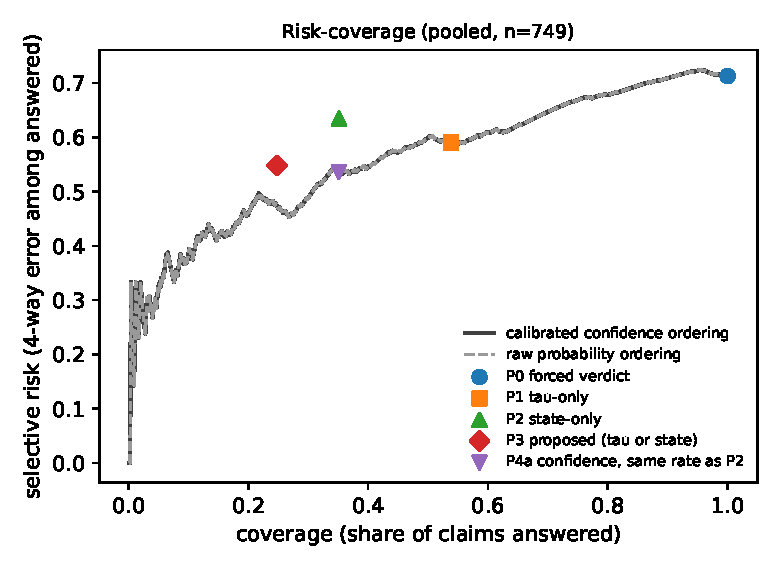
\includegraphics[width=0.56\linewidth]{figures/risk_coverage_pooled.pdf}
  \caption{Risk--coverage on the pooled evaluation claims. The curve orders claims by calibrated confidence; markers are the policies. State-only (P2) and the proposed policy (P3) lie above the confidence curve at their coverage.}
  \label{fig:rc}
\end{figure}

\runin{Mechanism check.} The test removes the state and replaces it with a confidence threshold that withholds the same fraction (P2 vs.\ P4a, P3 vs.\ P4b), holding data, classifier and counts fixed (Table~\ref{tab:mech}, Figure~\ref{fig:rc}). At \covPTwo\% coverage, state-only withholding has a \emph{higher} selective risk than the confidence threshold (\dRiskTwoFourA{} points, CI \dRiskTwoFourALo{} to \dRiskTwoFourAHi{}), with the same sign in both subsets (\dRiskTwoFourADev{} dev, \dRiskTwoFourATrain{} train). Unsafe errors do not differ detectably (\dUnsafeTwoFourA{} points, CI \dUnsafeTwoFourALo{} to \dUnsafeTwoFourAHi{}). The state also adds nothing about verdict correctness: AUROC is \aurocConf{} with confidence alone and \aurocConfState{} with the state added ($\Delta$ \dAuroc{}, CI \dAurocLo{} to \dAurocHi{}). Under the pre-set matrix, the state is \emph{redundant with calibrated confidence} in this pilot, plausibly because both derive from the same six counts. It is not uninformative on its own: verdicts are correct for \stateAccIns\% of claims in the \evs{Insufficient} state (\stateNIns{} claims) against \stateAccRef\% in \evs{Refutes}, and \refStateGoldR\% of \evs{Refutes}-state claims are gold R. Confidence captures the same information.

\begin{table}[t]
  \centering\small
  \caption{Mechanism check and baseline comparison: differences in percentage points (pooled).}
  \label{tab:mech}
  \begin{tabular}{@{}lccc@{}}
\toprule
Comparison (percentage points) & $\Delta$ coverage & $\Delta$ selective risk [95\% CI] & $\Delta$ unsafe errors [95\% CI] \\
\midrule
P3 $-$ P0 (proposed vs.\ baseline) & $-$75.2 & $-$16.5 [$-$22.5, $-$10.5] & $-$13.8 [$-$16.3, $-$11.5] \\
P2 $-$ P4a (state vs.\ confidence, same rate) & 0.0 & +9.9 [+4.2, +16.3] & +1.5 [$-$1.2, +3.3] \\
P3 $-$ P4b (proposed vs.\ confidence, same rate) & 0.0 & +7.5 [0.0, +15.1] & +1.3 [$-$0.4, +3.3] \\
\bottomrule
\end{tabular}

\end{table}

\runin{What this can and cannot establish.} At model level and on this slice, withholding reduces wrong decisive verdicts and the explicit state is not a better filter than calibrated confidence. It cannot show any effect on human decisions or trust, generalisation beyond this slice, or a causal effect of the state; C and N are too small (\nPoolC{} and \nPoolN{}) for inferential claims.

\runin{Variants and exploratory checks (disclosed).} After the freeze, an alternative answer prompt (v3) was tested on the tuning set only, under an adoption rule fixed beforehand (macro-F1 up by at least 0.02 and a higher Supports-vs-Refutes AUROC); it failed both (macro-F1 \vThreeDF{}, AUROC \vThreeDAUROC{}) and was not adopted. A guard bug in the evaluation driver was fixed after the tag without changing any number. An unplanned, exploratory check found that on the \postN{} claims with a decisive state, the rule ``Supports$\to$S, Refutes$\to$R'' is right \postRuleAcc{} of the time against \postClfAcc{} for the classifier, so the baseline is weak (\texttt{docs/DEVIATIONS.md}).

%==========================================================================
\section{Error Analysis, Trade-offs, Limitations and Ethics}\label{sec:limits}
%==========================================================================
\runin{Error analysis.} Of \unsafeErrTotal{} unsafe errors of the baseline, I sampled 8 per gold class (seeded) and read each with its questions, answers and snippets, assigning one type by hand (Table~\ref{tab:err}, Appendix~\ref{app:extra}). The labels are one annotator's, with no agreement statistic. The largest group is little usable evidence (\taxEv{} of \taxTotal{}): retrieval returns off-topic text, so most answers are Unverified (\unvPool\% of evaluation answers). For \taxEvGoldN{} of these the gold label is N, where little evidence is the right state and only the forced verdict is wrong. The next group is claims that are partly true or hinge on one detail, which six counts cannot express (\taxNua{}, of which \taxNuaGoldC{} are Conflicting). The rest are answerer misreads (\taxMis{}), classifier outputs contradicting counts that favour the other verdict (\taxClf{}), and off-topic or inverted questions (\taxDec{} and \taxPol{}).

\runin{Successes and failures.} \emph{Success 1:} ``Melissa Francis is married to Wray Thorn'' (gold S) is answered S and kept, but only two of ten answers are not Unverified and the snippets come from celebrity-gossip pages: correct yet fragile. \emph{Success 2:} a claim about the median wealth ratio (gold R, because the sources give averages) gets the right verdict R while the state says Supports, from a near-empty count vector (8 of 10 answers Unverified). \emph{Failure 1:} ``Raffia Arshad is the first hijab-wearing court judge'' (gold S) has the correct state Supports, but the classifier outputs R at confidence 0.78, overriding counts that favour support (3 supporting against 1 refuting answer). \emph{Failure 2:} for the claim that the Trump administration disbanded the pandemic response team (gold S) an inverted question (``retain key members?''$\to$No) is counted as refuting, and a retrieved page even carries a fact-checker's verdict line. Among the sampled N errors the state was \evs{Insufficient} in \nSampledNIns{} of \nSampledN{} cases while the forced verdict was wrong, which is the intended behaviour.

\runin{Who is underserved.} Baseline unsafe errors per gold class are \unsafeZeroS\% (S), \unsafeZeroR\% (R), \unsafeZeroC\% (C) and \unsafeZeroN\% (N); P3 withholds most claims in every class. Claims with scarce or conflicting evidence, subtle details, composite statements or opinions are served worst, and the excluded sensitive topics were never tested.

\runin{Trade-offs.} P3 gives up three quarters of the answers to reduce unsafe errors, and a confidence threshold gives a better risk--coverage trade-off than the state in this pilot (Figure~\ref{fig:rc}). On this evidence I would keep the abstention mechanism, but not claim a benefit for the explicit state until it is rebuilt on stronger evidence and shown to beat a confidence threshold.

\runin{Limitations.} Pilot slice (\nPool{} claims; one excluded after a failed decomposition); one 7B quantised model and prompt family, English only; retrieval is optimistic (store built from gold questions) yet still the bottleneck; no store dates and some residual fact-checking pages; broad exclusion filter; noisy gold labels; a pooled dev and train set, seen after this analysis; a weak baseline classifier (trained on \nTune{} claims); single-annotator error labels. No user study was run and no benefit to users is claimed.

\runin{Ethics and safeguards.} \emph{Privacy and data:} public claims from the dataset, some naming public figures, under CC BY-NC 4.0; no new personal data collected, no human participants, no credentials in code. \emph{Safety:} the state \evs{Insufficient} mostly reflects that retrieval found nothing usable, not that no evidence exists; it should be read as ``no usable evidence retrieved'', never as an assertion about the claim. A wrong \evs{Refutes} could unfairly label a speaker, so verdicts need human oversight. Withholding most verdicts also leaves most claims unchecked and shifts the work to human checkers, so abstention is a triage signal, not a safety guarantee. \emph{Misuse:} an automatic ``refuted'' stamp or automated moderation would misuse a system with macro-F1 \mfPool; sensitive topics were excluded and the exclusion bias is reported. \emph{Mitigation:} abstention, model-level framing only, frozen protocol, and full disclosure of variants.

%==========================================================================
\section{Reproducibility and Contribution Statements}\label{sec:repro}
%==========================================================================
Code, configuration, seeds, per-claim counts, predictions, tables and figures are in the code package (tag \texttt{stp1-frozen} plus later commits logged in \texttt{docs/DEVIATIONS.md}). The README gives the environment, data access and commands. \texttt{python -m src.run\_eval} regenerates every table and figure from the committed counts (about 25 seconds, no data or GPU), and every number in this report is a macro generated from \texttt{results/} by \texttt{src/make\_report\_tables.py}.

\runin{Contribution statement.} Individual project. Design, implementation, evaluation, analysis and writing: Taha Mehdi.

%==========================================================================
\bibliographystyle{ACM-Reference-Format}
\bibliography{refs}

\appendix
\section{Additional Results}\label{app:extra}
\begin{table}[h]
  \centering\small
  \caption{Technical metrics on the evaluation claims (baseline classifier, no abstention).}
  \label{tab:tech}
  \begin{tabular}{@{}lccc@{}}
\toprule
Metric & Pooled [95\% CI] ($n{=}749$) & Dev ($n{=}350$) & Train held-out ($n{=}399$) \\
\midrule
Accuracy & 0.287 [0.255, 0.319] & 0.329 & 0.251 \\
Macro-F1 & 0.225 [0.196, 0.256] & 0.260 & 0.194 \\
F1, Supports & 0.253 [0.190, 0.318] & 0.314 & 0.194 \\
F1, Refutes & 0.425 [0.379, 0.472] & 0.462 & 0.392 \\
F1, Conflicting & 0.114 [0.067, 0.165] & 0.156 & 0.080 \\
F1, Not Enough Evidence & 0.108 [0.043, 0.177] & 0.107 & 0.109 \\
ECE, raw confidence & 0.261 [0.232, 0.293] & 0.237 & 0.285 \\
ECE, calibrated confidence & 0.038 [0.030, 0.072] & 0.078 & 0.057 \\
Brier, calibrated & 0.701 [0.678, 0.724] & 0.716 & 0.687 \\
State accuracy & 0.236 [0.207, 0.266] & 0.269 & 0.208 \\
\bottomrule
\end{tabular}

\end{table}

\begin{table}[h]
  \centering\small
  \caption{Error types among the sampled unsafe errors (one hand-assigned type per case).}
  \label{tab:err}
  \begin{tabular}{@{}lr@{}}
\toprule
Error type & Cases (of 32) \\
\midrule
Evidence gap & 11 \\
Claim nuance beyond six counts & 8 \\
Answerer misreads snippet & 4 \\
Classifier contradicts clear counts & 3 \\
Off-topic or missing questions & 3 \\
Answerer too conservative & 1 \\
Gold label hard to defend & 1 \\
Question polarity or negation & 1 \\
\bottomrule
\end{tabular}

\end{table}

\begin{table}[h]
  \centering\small
  \caption{Evidence state versus verdict and gold label (pooled evaluation claims).}
  \label{tab:states}
  \begin{tabular}{@{}lrrrr@{}}
\toprule
Predicted state & Claims & Share (\%) & Verdict correct (\%) & Gold S / R / C / N \\
\midrule
Supports & 188 & 25.1 & 31.4 & 72 / 90 / 15 / 11 \\
Refutes & 75 & 10.0 & 49.3 & 4 / 61 / 4 / 6 \\
Mixed & 121 & 16.2 & 51.2 & 36 / 75 / 7 / 3 \\
Insufficient & 365 & 48.7 & 15.6 & 89 / 215 / 24 / 37 \\
\bottomrule
\end{tabular}

\end{table}

\begin{figure}[h]
  \centering
  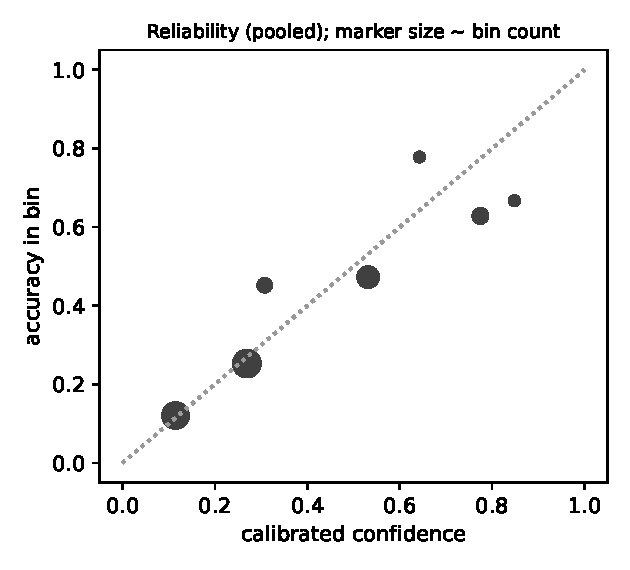
\includegraphics[width=0.55\linewidth]{figures/reliability_pooled.pdf}\hfill
  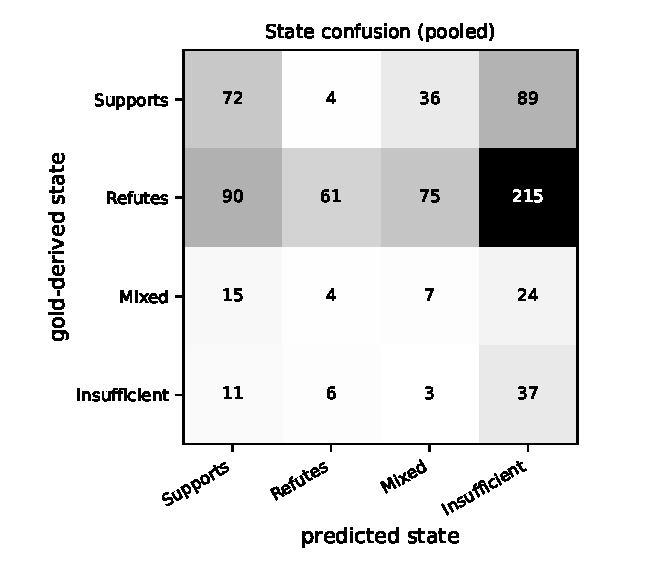
\includegraphics[width=0.40\linewidth]{figures/state_confusion_pooled.pdf}
  \caption{Left: reliability of raw and calibrated confidence. Right: predicted evidence state against the state implied by the gold label.}
\end{figure}

\end{document}
